% Note: The examples have been moved to the previous section in order to appear on p. 2.

\section{A new corpus for NLI}\label{sec:discussion}

To date, the primary sources of annotated NLI corpora have been the
Recognizing Textual Entailment (RTE)
challenge tasks.\footnote{\url{http://aclweb.org/aclwiki/index.php?title=Textual_Entailment_Resource_Pool}}
These are generally high-quality, hand-labeled data sets, and they
have stimulated innovative logical and statistical models of natural
language reasoning, but their small size (fewer than a thousand examples each)
limits their utility as a testbed for learned distributed representations. 
The data for the SemEval 2014 task called Sentences Involving Compositional Knowledge (SICK) is a
step up in terms of size, but only to 4,500 training examples, and its
partly automatic construction introduced some spurious patterns into
the data (\citealt{marelli2014semeval}, $\S$6). Finally, the
Denotation Graph entailment set \cite{hodoshimage} contains millions of
examples of entailments between sentences and artificially constructed
short phrases, but it was labeled using fully automatic methods, and is
noisy enough that it is probably suitable only as a source of
supplementary training data. The Paraphase Database of \newcite{ganitkevitch2013ppdb}
addresses these issues of size and quality, but only for the limited
fragment of the NLI problem that is captured by paraphrase.

Existing resources suffer from a subtler issue that impacts even
projects using only human-provided annotations: indeterminacies of
event and entity coreference lead to insurmountable indeterminacy
concerning the correct semantic label (\citealt{de2008finding} $\S4.3$; \citealt{marelli2014sick}). For
instance, the sentence pair \word{A boat sank in the Pacific
  ocean} and \word{A boat sank in an ocean} could reasonably be labeled in
numerous ways depending on how the objects and events are grounded. If
the two boats are assumed to be different, then the sentences are semantically
independent. If the boats and the oceans are assumed to be the same,
then the first sentence entails the second (in the relevant
commonsense way). If the boats are assumed to be the same and 
\word{an ocean} in the second sentence is interpreted with a specific referent 
that is not the Pacific, then the two events are (commonsense) contradictory. This
kind of indeterminacy can be resolved only once the questions of
coreference are resolved.


With our corpus, we sought to address the issues of size, quality, and
indeterminacy. To do this, we employed a crowdsourcing framework with
the following crucial innovations. First, the examples were grounded
in specific scenarios, and the premise and hypothesis sentences in each example 
were constrained to describe that scenario from the same perspective, 
which helps greatly in controlling event and entity coreference. Second, the prompt
gave participants the freedom to produce entirely novel sentences
within the task setting, which led to richer examples than we see with
the more proscribed string-editing techniques of earlier approaches,
without sacrificing consistency. Third, a subset of the resulting
sentences were sent to a validation task aimed at providing a highly 
reliable set of annotations over the same data, and at identifying areas of inferential uncertainty.

% Our ultimate aim in this work is to develop supervised models for sentence representation that can accurately capture natural language meaning. While sentiment tasks like SST have provided a useful testbed for sentence representation models, sentiment labeling only requires that models be able to encode a small piece of the full expressive capacity of language. We claim that the task of natural language inference (also called recognizing textual entailment, or RTE) is significantly more demanding, and that strong performance on this task is good evidence of a model's overall strength in sentence representation.

% \subsection{Grounding with imagined images}

% \todo{Rewrite and expand (CP?)} --- I incorporated this above.

% Quote from SICK paper \cite{marelli2014sick}:

% \begin{quote}
% Not unreasonably, subjects found that, say, \ii{A woman is wearing an Egyptian headdress} does not contradict \ii{A woman is wearing an Indian headdress}, since one could easily imagine both sentences truthfully uttered to refer to a single scene where two different women are wearing different headdresses. In the future, a higher proportion of CONTRADICTION labels could be elicited by using grammatical and possibly visual cues (pictures) encouraging co-indexing of the entities in the two sentences.
% \end{quote}

%\todo{SICK is referenced below, so we should set it up as a point of reference either here or in the intro, including mentioning that it had both entailment and similarity labels.}

\subsection{Data collection}

\begin{figure}
\begin{framed}
\small
We will show you the caption for a photo. We will not show you the photo. Using only the caption and what you know about the world:
\begin{itemize}
\item Write one alternate caption that is \textbf{definitely} a \textbf{true} description of the photo. \ii{Example: For the caption ``\ii{Two dogs are running through a field.}'' you could write ``\ii{There are animals outdoors.}"}
\item Write one alternate caption that \textbf{might be} a \textbf{true} description of the photo. \ii{Example: For the caption ``\ii{Two dogs are running through a field.}" you could write ``\ii{Some puppies are running to catch a stick.}"}
\item Write one alternate caption that is \textbf{definitely} a \textbf{false} description of the photo. \ii{Example: For the caption ``\ii{Two dogs are running through a field.}" you could write ``\ii{The pets are sitting on a couch.}" This is different from the} maybe correct \ii{category because it's impossible for the dogs to be both running and sitting.}
\end{itemize}
\end{framed}

\caption{\label{instructions-1}The instructions used on Mechanical Turk for data collection.}
\end{figure}

We used Amazon Mechanical Turk for data collection. In each individual task (each HIT), a worker was presented with premise scene descriptions from a preexisting corpus, and asked to supply hypotheses for each of our three labels---\ii{entailment}, \ii{neutral}, and \ii{contradiction}---forcing the data to be balanced among these classes.

The instructions that we provided to the workers are shown in \reffig{instructions-1}. Below the instructions were three fields for each of three requested sentences, corresponding to our \ii{entailment}, \ii{neutral}, and \ii{contradiction} labels, a fourth field (marked optional) for reporting problems, and a link to an FAQ page. That FAQ grew over the course of data collection. It warned about disallowed techniques (e.g., reusing the same sentence for many different prompts, which we saw in a few cases), provided guidance concerning sentence length and complexity (we did not enforce a minimum length, and we allowed bare NPs as well as full sentences), and reviewed logistical issues around payment timing. About 2,500 workers contributed.


For the premises, we used captions from the Flickr30k corpus \cite{hodoshimage}, a collection of approximately 160k captions (corresponding to about 30k images) collected in an earlier crowdsourced effort. The captions were not authored by the photographers who took the source images, and they tend to contain relatively literal scene descriptions that are suited to our approach, rather than those typically associated with personal photographs (as in their example: \word{Our trip to the Olympic Peninsula}).

\Reftab{collection-stats} reports some key statistics about the collected corpus, and \reffig{length-dist} shows the distributions of sentence lengths for both our source hypotheses and our newly collected premises. We observed that while premise sentences varied considerably in length, hypothesis sentences tended to be as short as possible while still providing enough information to yield a clear judgment, clustering at around seven words.

\begin{table}
\center
  %\setlength{\tabcolsep}{15pt}
  %\renewcommand{\arraystretch}{1.2}
  \begin{tabular}{l l} 
    \toprule
\multicolumn{2}{l}{\textbf{Data set sizes:}}\\
Training pairs &  550,152\\
Development pairs &  10,000\\
Test pairs & 10,000\\
\midrule
\multicolumn{2}{l}{\textbf{Sentence length:}}\\
Premise mean token count & 14.1\\
Hypothesis mean token count & 8.3 \\
\midrule
\multicolumn{2}{l}{\textbf{Parser output:}}\\
Premise `S'-rooted parses & 74.0\%\\
Hypothesis `S'-rooted parses & 88.9\%\\
Distinct words (ignoring case) & 37,026\\
    \bottomrule
  \end{tabular}
% From 1.0rc3
\caption{\label{collection-stats}Key statistics for the raw sentence pairs. Since the two halves of each pair were collected separately, we report some statistics for both.} 
\end{table}


\begin{figure}
\center
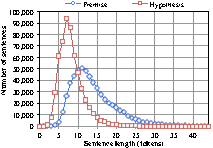
\includegraphics[width=3.05in]{length_dist}
    % From 1.0rc2, though still accurate as of rc3
% \todo{Replace w/ mean+SD if low on space.}
\caption{\label{length-dist}The distribution of sentence length.} 
\end{figure}

\subsection{Data validation}

In order to measure the quality of our corpus, and in order to construct maximally useful testing and development sets, we performed an additional round of validation for about 10\% of our data.
This validation phase followed the same basic form as the Mechanical Turk labeling task used to label the SICK entailment data: we presented workers with pairs of sentences in batches of five, and asked them to choose a single label for each pair. We supplied each pair to four annotators, yielding five labels per pair including the label used by the original author. The instructions were similar to the instructions for initial data collection shown in \reffig{instructions-1}, and linked to a similar FAQ. Though we initially used a very restrictive qualification (based on past approval rate) to select workers for the validation task, we nonetheless discovered (and deleted) some instances of random guessing in an early batch of work, and subsequently instituted a fully closed qualification restricted to about 30 trusted workers.

For each pair that we validated, we assigned a gold label. If any one of
the three labels was chosen by at least three of the five annotators, it was 
chosen as the gold label. If there was no such consensus, which
occurred in about 2\% of cases, we assigned the placeholder label `-'. 
While these unlabeled examples are included in the corpus distribution, they are
unlikely to be helpful for the standard NLI classification task, and
we do not include them in either training or evaluation in the experiments that we 
discuss in this paper. 

The results of this validation process
are summarized in \reftab{validation-stats}. 
Nearly all of the examples received a majority
label, indicating broad consensus about the nature of the data and
categories. The gold-labeled examples are very nearly evenly
distributed across the three labels. The Fleiss $\kappa$ scores 
(computed over every example with a full five annotations)
are likely to be conservative given our large and
unevenly distributed pool of annotators, but they still provide insights
about the levels of disagreement across the three semantic
classes. This disagreement likely reflects not just the limitations of
large crowdsourcing efforts but also the uncertainty inherent in naturalistic NLI.
Regardless, the overall rate of agreement is extremely high,
suggesting that the corpus is sufficiently high quality to pose a
challenging but realistic machine learning task.

\begin{table}
\center
  %\setlength{\tabcolsep}{15pt}
  %\renewcommand{\arraystretch}{1.2}
  \begin{tabular}{l l} 
    \toprule
\multicolumn{2}{l}{\textbf{General:}}\\
Validated pairs & 56,951\\
Pairs w/ unanimous gold label & 58.3\%\\
\midrule
\multicolumn{2}{l}{\textbf{Individual annotator label agreement:}}\\
Individual label $=$ gold label & 89.0\%\\
Individual label $=$ author's label & 85.8\%\\
\midrule
\multicolumn{2}{l}{\textbf{Gold label/author's label agreement:}}\\
Gold label $=$ author's label & 91.2\%\\
Gold label $\ne$ author's label & 6.8\% \\
No gold label (no 3 labels match) & 2.0\%\\
\midrule
\multicolumn{2}{l}{\textbf{Fleiss $\kappa$:}}\\
    \ii{contradiction} & 0.77 \\
    \ii{entailment} & 0.72 \\
    \ii{neutral} & 0.60 \\
    Overall & 0.70 \\
    \bottomrule
  \end{tabular}
    % From 1.0rc3
\caption{\label{validation-stats}Statistics for the validated pairs. The \ii{author's label} is the label used by the worker who wrote the premise to create the sentence pair. A \ii{gold label} reflects a consensus of three votes from among the author and the four annotators.} 
\end{table}

\subsection{The distributed corpus}

\Reftab{snli-examples} shows a set of randomly chosen validated examples from the development set with their labels. Qualitatively, we find the data that we collected draws fairly extensively on commonsense knowledge, and that hypothesis and premise sentences often differ structurally in significant ways, suggesting that there is room for improvement beyond superficial word alignment models. We also find the sentences that we collected to be largely fluent, correctly spelled English, with a mix of full sentences and caption-style noun phrase fragments, though punctuation and capitalization are often omitted.

The data will be released upon publication under a CreativeCommons
Attribution-ShareAlike license, the same license used for the Flickr30k source captions.


\paragraph{Partition} 

We distribute the corpus with a pre-specified train/test/development split. The test and development sets contain 10k examples each. Each original ImageFlickr caption occurs in only one of the three sets, and all of the examples in the test and development sets have been validated.

\paragraph{Parses}

The distributed corpus includes parses produced by the Stanford PCFG Parser 3.5.2 \cite{klein2003accurate}, trained on the standard training set as well as on the Brown Corpus (\citealt{francis1979brown}), which we found to improve the parse quality of the descriptive sentences and noun phrases found in the descriptions. 

% Parses are available in both the standard PTB format and in the binarized unlabeled format used by tree-structured neural network models.

%\paragraph{General evaluation standards}
%While we hope that the corpus will be valuable in a variety of ways, we encourage researchers working on tools for semantic representation and inference to evaluate on our data in a uniform way: training on only the (parsed and/or unparsed) sentences included in the training set, and doing final evaluations on only the subset of the test set for which there are single gold labels.
